\chapter[Manufacturing, layouts and metrics]{Manufacturing, production layouts and related metrics}
\vspace{-0.5cm}
\minitoc

\begin{quotation}
    \textsf{\noindent\textbf{Manufacturing} can be seen as the process which turns starting material into completed/finished products. In this chapter a \textit{classification for industries and products}, a taxonomy of classical operations in manufacturing, a \textit{classification of typical facilities layouts} is made.}
\end{quotation}
From a \textbf{technological point of view} the manufacturing \underline{process} is the application of machinery, tools, power and labor in order to convert some \textit{starting material}\footnote{
    In some cases, these are raw materials
} into \textit{completed part} also known as \textit{products}. There is another \textbf{economic definition} which focuses on the fact that by performing the processing transforming starting material into values, the manufacturing \textbf{adds value} to them. Common examples can be made: into transforming sand into glass, manufacturing adds value; into transform iron in steel, value is added and so on.

\begin{figure}[h]
    \centering
    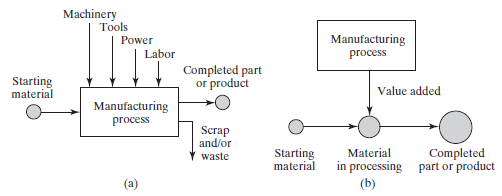
\includegraphics[scale=1]{img/manifacturing.png}
    \caption{Manufacturing: economic and technological views}
    \label{fig:manifacturing_views}
\end{figure}
  

\section{Manifacture industries and products}
The types of operations involved in the manufacturing process depend on the products a certain factory produces. All of the insustries can be in general classified as:
\begin{enumerate}
    \itemsep-0.3em
    \item \textit{Primary Industries} they exploit natural resources and materials. Examples of such activities are the agricolture and the mining; 
    \item \textit{Secondary Industries} convert primary industries materials into products; 
    \item \textit{Tertiary Industries} is the service sector of the economics.
\end{enumerate}
A further distinction about industries can be made according to the type of products they do. In particular, we can distinguish between \textbf{process industries} like chemicals and energy and those industries which produces \textbf{discrete parts and products}. The production operationn can be divided into \textit{continuous production} and \textit{batch production}. In the former case the equipment is used exclusively for the fiven product and the output of the process is \underline{uninterrupted}. In the latter case, starting materials are  processed in finite amount or quantities. Such finite amount is called \textbf{batch}. Differently from the first case, batch production is discontinuous because there can be interruptions between batches. This distintion is valid for both continuous and discrete manufacturing industries. The figure \Cref{fig:mani_classes} depicts schematically the distinction we have just introduced here.

\begin{figure}[h]
    \centering
    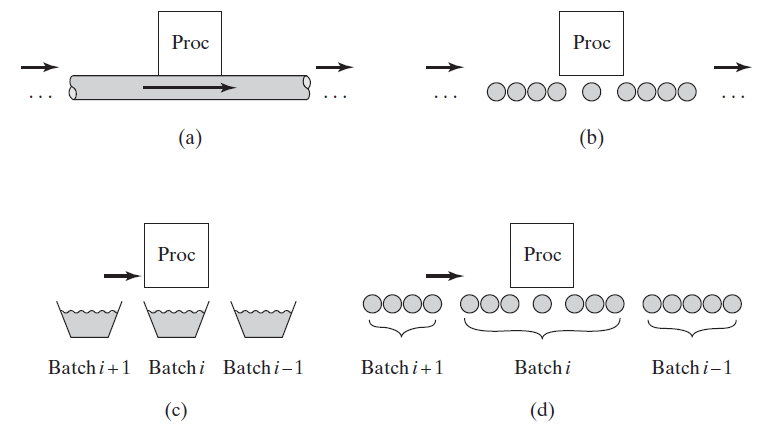
\includegraphics[scale=0.7]{img/mani_classification.png}
    \caption{(Process/Discrete) vs (Continuous/Batch) production}
    \label{fig:mani_classes}
\end{figure}

\section{Manufacturing operations}
What is inside the box depicted as \textit{Manufacturing process} in \Cref{fig:manifacturing_views}? There are some basic activities that must be executed in order to transform raw materials into products. In particular they are: (1) Processing and Assembly operations, (2) Material handling operations, (3) Inspection and tests, (4) operations involving coordination and control.

\subsection{Processing and Assembling}
These are two subclasses of manufacturing process. \textbf{\textit{Processing operations}} deal with transforming raw material from one initial state to another which is \textit{closer to the final state}. How it happens for other operations, value is added and in particular the shape, geometry and other properties are changed. On the other hand, \textbf{\textit{Assembling operations}} are in order to put together more elementary parts with the aim of creating \textbf{new entities} which sometimes is called \textit{assembly} or \textit{subassembly}. We can add that the different parts are connected together either permanently (eg. soldering) or in a way that at a certain point can be disassembled. This technique for assembling is referred as \textit{semipermanent}.\\
The figure \Cref{fig:man_breakdown} shows a complete classification of processing and assembling operations.

\begin{figure}
    \centering
    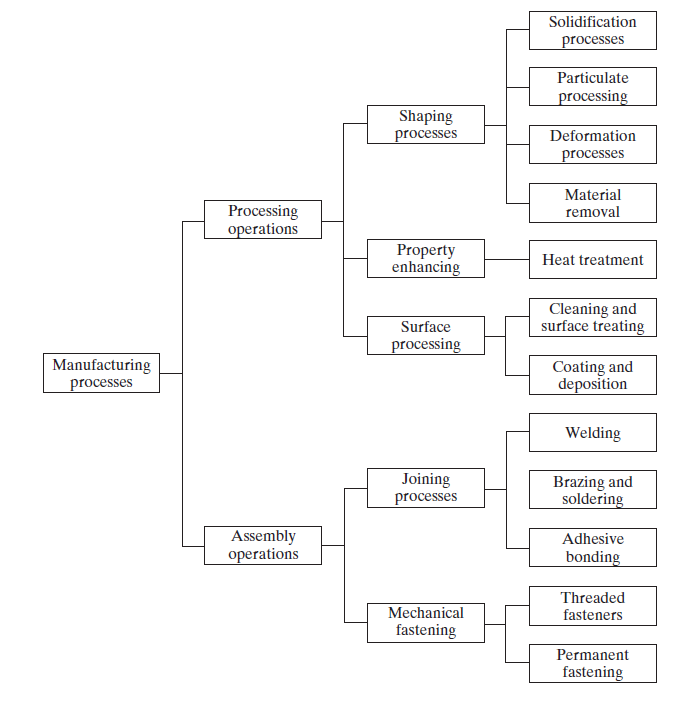
\includegraphics[scale=1]{img/man_processes.png}
    \caption{Manufacturing processes breakdown}
    \label{fig:man_breakdown}
\end{figure}

\subsection{Material handling}
\textbf{Material handling} concerns with those operations which are finalized to moving parts and materials between processing or assembling operations. A famous advocate, in a study observed that materials in a typical industry spent the great majority of their time to be moved and properly stored (tipically the 95\% of the time a typical part (for batch production) passes its time moving or on shelves).
\subsection{Inspection and test}
Both \textbf{inspection} and \textbf{testing} are \textit{quality control activities} they are in order to decide whether the products respect standard and specification. More specifically, when one talks about \textit{inspection} examines if the single parts of a certain object are within the tolerances dictated by the engineering drawing of the part itself. The \textit{test} is more referred as testing the \textbf{functionalities} of the final product rather than the single pieces constituting them. 

\subsection{Coordination and control}
These are all those operation involving plant-level activities. The difference is that here we are talking about support functions, while the first three basic basic activities "touch" in some way either the starting material or the final products.

\section{Production facilities and Manufacturing layouts}
The way a certain factory decides  to organize their facilities depend on the type, variety and quantities of pieces, the factory itself can produce. It could seem trivial, but such factors influence a lot the way the facilities can be organized in order to optimize the production. The \textsf{number of products a given plant produces annually} is called \textbf{production quantity}. They can be classified into three ranges (namely \textit{small, medium and high} production) whose breakpoint are reported in the figure and are in some sense overlapped. Another important parameter is the \textbf{product variety} which, in a quantitative way, can be seen as the number of different products the plant can produce. As you can see in the \Cref{fig:quantity_variety} there is a sort of inverse correlation between the two aspects. The higher the variety the lower the annual quantity of produced items.\\
While the production quantity is a well-quantifiable parameter it is not trivial to give exact numbers on the variety. A mean to introduce a sort of quantifiable distinction is the following criterium: how many differences there are between one product and another? In this context we are referring to \textbf{hard variety} (there are substancial differences between products) and \textbf{soft variety} (small differences like the ones are made on producing cars).\\
\begin{figure}
    \centering
    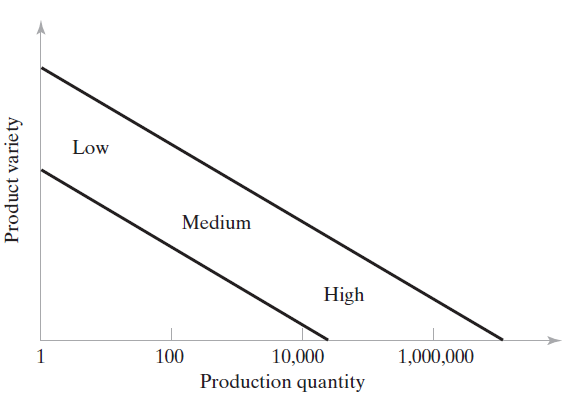
\includegraphics[scale=1]{img/quantity_variety.png}
    \caption{Quantity vs Variety plot}
    \label{fig:quantity_variety}
\end{figure}

The Production quantity parameter, moreover, is used in order to individuate \textbf{three basic categories} of production plants.

\subsection{Low Production (1-100 units)}
The type of production plant associated with low production is said \textbf{job-shop}. The type of products are tipically very complex (for example aircraft, heavy machinery), workers are highly specialized in doing some tasks. In order to tackle the dimensions of such products, they are always in the same position, while moving toward them workers and equipment. This type of layout is known as \textbf{fixed layout}. In the practice such products are assembly of large modules made at single location.\\
The individual parts are built in factories whose plant has got a \textbf{process layout} where, basically, equipment is arranged according to its type or function, moreover workers and the equipment they use are arranged in \textit{departments} specialized with a single function. The main advantage of the process layout is the \textit{flexibility} since operations do not have to follow a fixed sequence. At the opposite, more intense \textit{moving/handling} operations are needed to move intermediate artifacts from one department to another.
\subsection{Medium production (100-10000 units)}
For medium production quantity we can have basically two types of production plants according to the variety for the products. In particular for hard variety we have a \textbf{batch production} parts are produced in batches that are later furthermore elaborated (a changeover time is required in order to pass from one step to another). A suitable layout for such a type of plant is the just seen process layout. At the opposite, when you have soft variety for products the equipment (computers and machine) can be organized in cells. Here similar parts/products can be made on the same machinery without a significant time loss for changeover. This is called a \textbf{cellular layout}.

\subsection{High production(10000-1000000 units)}
We also refer it as \textbf{mass production}, moreover two categories can be distinguished: \textit{quantity production} and \textit{Flow-line production}. \textbf{Quantity production} is referred as the production of single parts on single pieces the equipment is specialized in the production of one part type, the classical layout is the process layout. In \textbf{Flow-line production} we have multiple workstations \underline{arranged in a sequence} here materials or assemblies are moved through the sequence in a way that \textit{step-by-step} the final product is obtained. Since the sequence of machines is organized according to the product, this is known as \textbf{product layout}.

\begin{figure}[h]
    \centering
    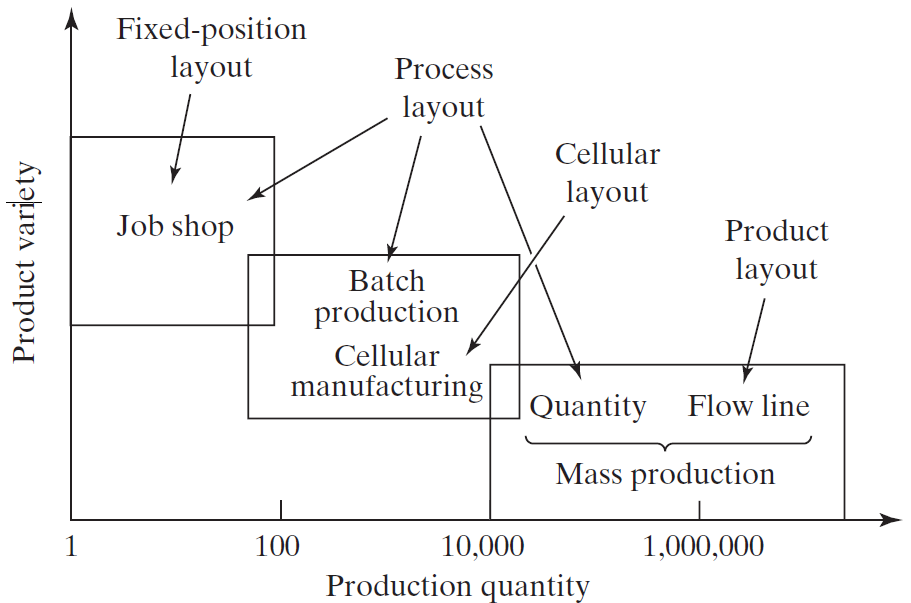
\includegraphics[scale=0.5]{img/layouts_plants.png}
    \caption{Production plants and related layouts}
\end{figure}

The figure above summarizes most of the discussion we had on facilities and their layout.

\begin{figure}
    \centering
    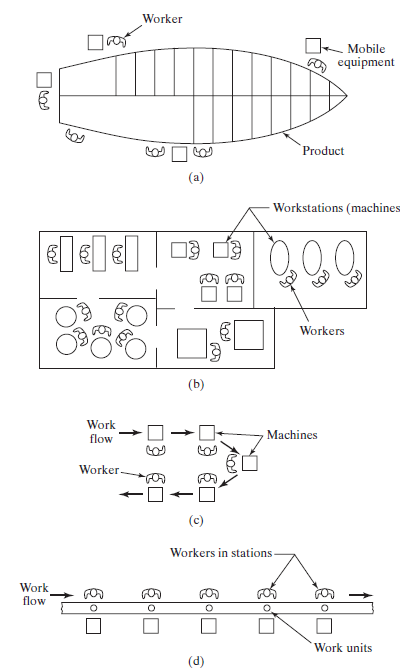
\includegraphics[scale=1.2]{img/plant_layouts.png}
    \caption{(a) fixed layout, (b) process layout, (c) cellular layout, (d) product layout}
\end{figure}

\section{Product/Production relationship}
In the first part of this chapter we have seen that the factories organize their facilities in the most efficient manner according the products they produce. It is particularly useful to observe that there are certain product parameters which are relevant for manufacturing. In particular: (1) production quantity, (2) production variety, (3) product complexity, (4) part complexity. 

\subsection{Production quantity and product variety}
\textit{Production quantity and variety} are important parameters which have been discussed previously. We indicate them respectively with $Q$ and $P$. We can indicate with $Q_j$ the quantity for parts or product of a certain style $j$ while $Q_f$ is the total amount of products/parts ofer all the styles: 
\begin{equation}
    Q_f=\sum_{j=1}^P {Q_j}
\end{equation}
where $P$ is the number of styles of products/parts. The parameter $P$ is related to the product variety and  in order to better embed the concepts of hard/soft variety we can divide it into two sublevels: $P_1$ is the number of different product lines, $P_2$ is the number of styles for that product line. In this way the total number of models is given by: 
\begin{equation}
    P=\sum_{j=1}^{P_1}{P_{2j}}
\end{equation}

\subsection{Product and part complexity}
Stating something about the complexity of the production is a non-trivial task since they involve both quantitative and qualitative aspects. However, for assembled products the complexity can be seen as the number of components, while for a manifactured part, complexity can be explained by the number of operations that product requires. 
The tables in \Cref{fig:part_complexity} and \Cref{fig:prod_complexity} shows examples of number of processing stages and number of components, respectively, for parts and products.

\begin{figure}
    \centering
    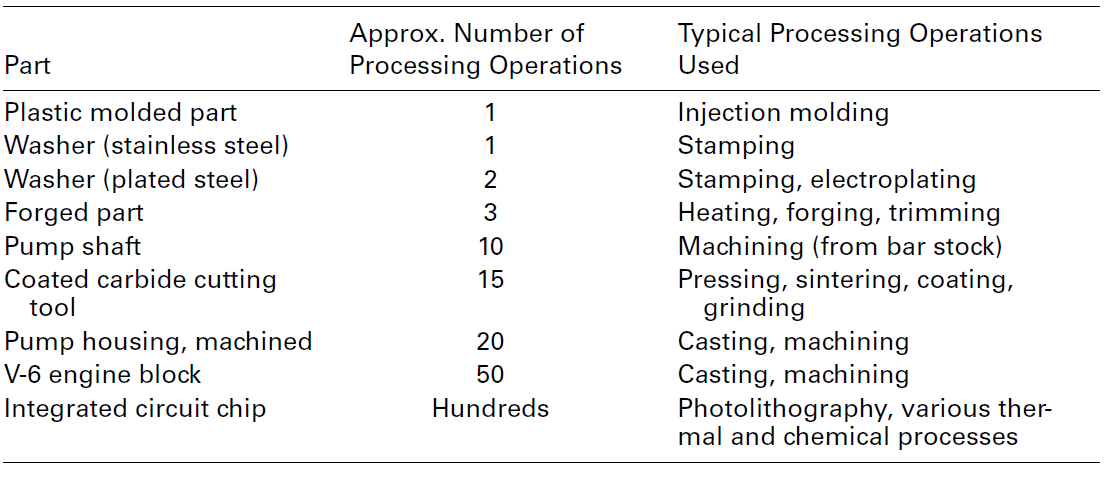
\includegraphics[scale=0.6]{img/part_complexity_table.png}
    \caption{Part complexity}
    \label{fig:part_complexity}
\end{figure}

\begin{figure}
    \centering
    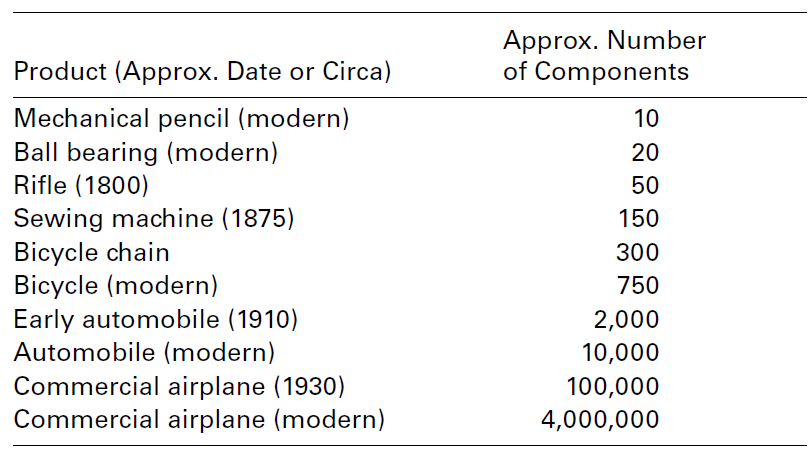
\includegraphics[scale=0.6]{img/prod_complexity_table.png}
    \caption{Product complexity}
    \label{fig:prod_complexity}
\end{figure}

In the following we will call $n_p$ and $n_o$ the number of parts of which is composed a certain product and the number of operations a certain part requires.
From both $n_p$ and $n_o$ can be obtained a classification for industries which is given in \Cref{fig:npno}.

\begin{figure}
    \centering
    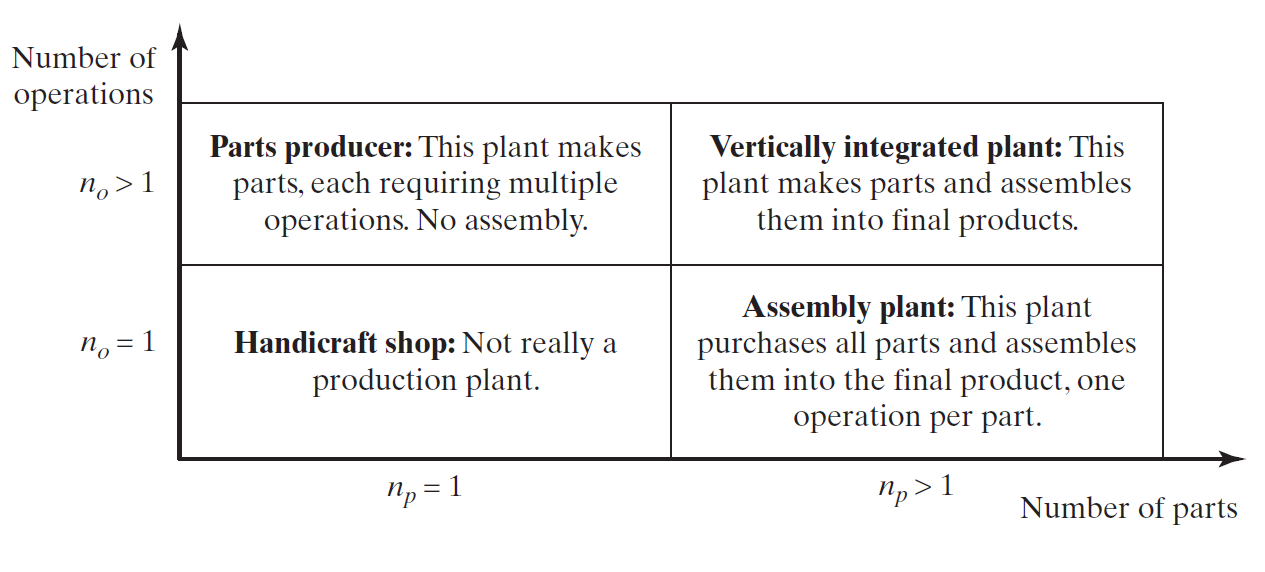
\includegraphics[scale=0.6]{img/np_vs_no.png}
    \caption{Production plants distinction according $n_p$ and $n_o$}
    \label{fig:npno}
\end{figure}

There are several relationships can be obtained from $Q,P,n_o,n_p$, here we are ignoring the diffeerence between $P_1$ and $P_2$. The \Cref{tab:prod_param} reports them. Average values of the four parameters $Q, P, n_o, n_p$ could be used to simplify the factory model.

\begin{align}
    &Q_f=PQ\qquad Q=\frac{\sum_{j=1}^P {Q_j}}{P}\\
    &n_{pf}=PQn_p \qquad{n_p}=\frac{\sum_{j=1}^{P}{Q_j{n_{pj}}}}{PQ}\\
    &n_{of}=PQn_p{n_o}\qquad n_o=\frac{
        \sum_{j=1}^{P}Q_j\sum_{k=1}^{n_{pj}}{n_{ojk}}
    }{PQn_{pf}}
\end{align}


\begin{table}
    \centering
    \begin{tabular}{p{5cm} p{10cm}}
        \toprule
        \textbf{Parameter}&\textbf{Description}\\
        \toprule\toprule
        {$Q_f$, $Q_j$}&{Total product/parts produced annually and total product/parts of a certain style}\\
        \midrule
        {$n_p$, $n_o$}&{Number of parts for a product (assembly), number of operations for obtaining a certain part}\\
        \midrule
        $n_{pf}=\sum_{j=1}^{P}{Q_j{n_{pj}}}$&{Total number of parts manifactured by the plant}\\
        \midrule
        {$n_{of}=\sum_{j=1}^{P}Q_j\sum_{k=1}^{n_{pj}}{n_{ojk}}$}&{Total  number of operatisn required for all the parts for all the products. Here $n_{ojk}$ is the number of operations for a certain part $k$ of a certain style $j$}\\ 
        \bottomrule
        \bottomrule
     \end{tabular}
     \caption{Product parameters}
     \label{tab:prod_param}
\end{table}

\section{Limitations of manufacturing plants}
An important aspect to consider is that a manifacturing plant cannot do everything! Often we find the name of \textit{focused factories} to indicate \textit{"on a limited, coincise, manageable set of products, technologies, volumes and markets"}. The objective is then \textbf{limiting the scope} of the factory. The most immediate way is avoiding making a fully integrated factory, being a parts producer or an assembly plant is better. In general, all these concepts can be summarized with the term \textbf{manifacturing capability} which is the  
\begin{quotation}
    \textit{technical and physical limitatioins of a manifacturing firm and of each plants}
\end{quotation}

\section{Manifacturing metrics and economics}
How we have seen in the introduction quantitative metrics allow to estimate performances of the plant, individuate issues, estimating costs for products and parts. Metrics can be divided in two groups: (i) production performance metrics, (ii) manifacturing costs.
\subsection{\color{red} Production performance metrics}
\subsubsection{Cycle time: $T_c$ (min)}
For a single operation (one step) the cycle time $T_c$ is the time that a product/part (work unit) \underline{spends being processed or assembled}. This is nothing but the time elapsing between the beginning of the processing of a product and the beginning of the next piece. Tipically the cycle time is: 

\begin{equation}
    T_c=T_o+T_h+T_t
\end{equation}
where $T_c$ is given in min/pc, $T_o$ is the actual processing or assembling operation, $T_h$ is the handling time while $T_t$ is the tooling time which is the time spent in changing from one tool to another.

\subsubsection{Production rate: $R_p$ [pc/hr]}
For a single operation the \textit{production rate} is the number of  work units completed in a hour. Such a metric $R_p$ changes according to the type of production we are considering. Mainly the steps are: (i)obtaining an expression for the production time (min/pc), (ii) inverting it for obtaining $R_p$ (pcs/hr). The different situations arising here are: 
\begin{itemize}
    \itemsep-0.3em
    \item \textit{Job shop}. Considering the case when $Q=1$, the \textbf{production time} is the sum of the setup time and the cycle time, that is: 
    \begin{equation}
        T_p=T_{su}+T_c
    \end{equation}
    where the \textbf{setup time} $T_{su}$ is the time for preparing the machine in producing that part.
    In this case the production rate (in pc/hr) is given by 
    \begin{equation*}
        R_p=\frac{60}{T_p}
    \end{equation*}
    \item \textit{Batch processing}. Here we have to make a further distinction for pieces of the batch that are processed one at a time and the ones which are processed all together. In the former case we have that the time for processing a batch is $T_b=T_{su}+Q{T_c}$ in the latter case we have $T_b=T_{su}+T_{c}$. The average production time per unit is given by 
    \begin{equation}
        T_p=\frac{T_b}{Q}
    \end{equation}
    where $Q$ is the batch-size, the production rate is computed as before.
    \item \textit{Mass production}. We have distinguished \textit{quantity mass production} and \textit{flow-line mass production}. We have different formulas for the two cases. In the first case since $Q$ becomes very large the production rate $R_p$ tends to be the \textbf{cycle rate} $R_c$ since the setup becomes negligible with the increasing quantity
    \begin{equation}
        R_c=\frac{60}{T_c}
    \end{equation}
    For flow-line production the discussion is a bit more complicated since multiple workstations are involved. At first we can say that the same holds concerning $R_p$ which becomes $R_c$. But, what about $T_c$, the cycle time for processing a single part/product is dominated by the \textbf{operation time of the slowest machine} to which is added the time $T_r$ to transfer the pieces between work units. Summarizing:
    \begin{equation}
        T_c= \max{T_o} + T_r
    \end{equation}
    remind that $T_c \to (min/pc)$. At this point the cycle rate can be obtained as usual.
\end{itemize}

\begin{figure}
    \centering
    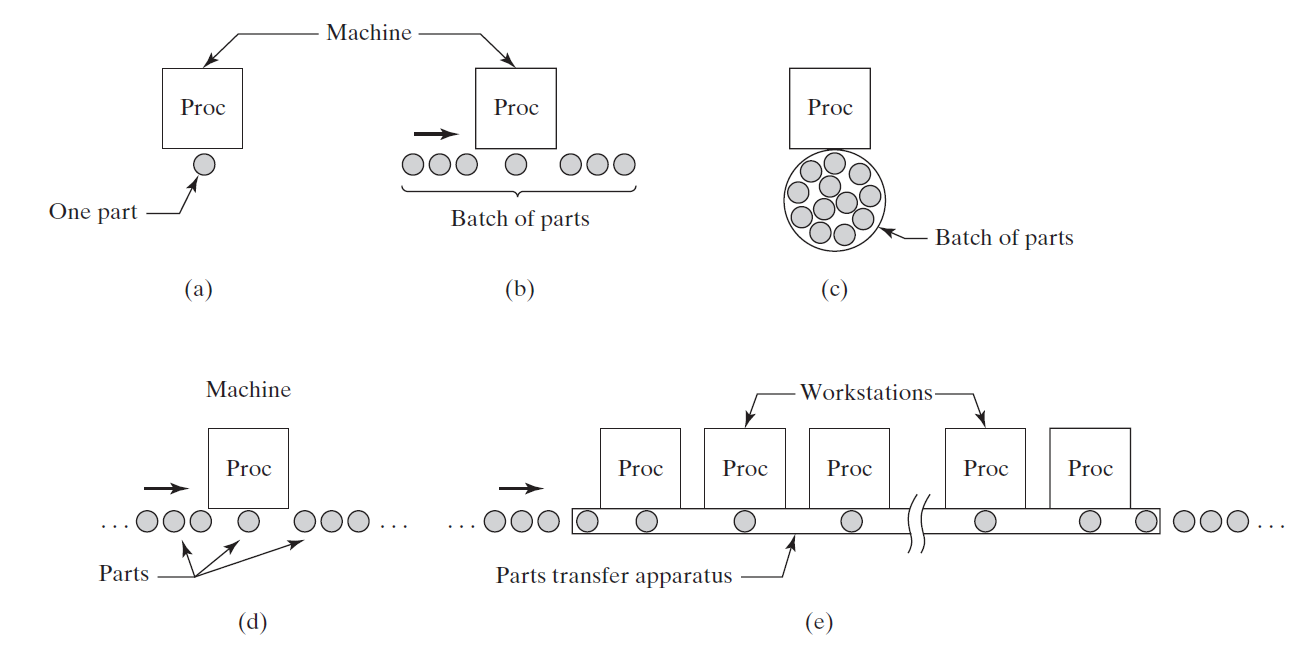
\includegraphics[scale=0.6]{img/production_rates.png}
    \caption{Different production plants for considering production rates}
\end{figure}

\subsubsection{Equipment reliability: availability}
Till now, we have considered the different ways by which computing the production rates in the ideal case, that is ignoring the lost time due to the \textit{equipment reliability}. The metric we can use for reliability is the \textbf{availability} which is defined as the portion of the time the equipment works correctly. In turn, the availability $A$ is defined according other two metrics (MTBF, Mean Time Between Failure and MTTF, Mean Time to failure). The exact formula is: 
\begin{equation}
    A=\frac{MTBF-MTTR}{MTBF}
\end{equation}
the average production rate is obtained by multiplying the $R_p$ by the availability. This is the same to say that in the non-ideal condition the production rate is reduced according to the availability of a certain machine.

\subsubsection{Plant Capacity ($PC$)}
The production capacity is defined as the \textbf{maximum rate of output} that a plant can produce \underline{under a set of operating conditions} such as: number of shifts per day (1-3), number of days in the week... The operating conditions are not trivial to determine. Suppose you have $n$ machines producing the same part and having the same production rate $R_p$, the production rate in this case is given by 
\begin{equation}
    PC={n}{H_{pc}}{R_p}
\end{equation}
where $H_{pc}$ is the amount of hour in the period and $PC$ is measured in (pc/period). The period can be for example a week, a month, a year... A slightly more complex situation arises when the $n$ machines have different production rates, but all can work for $Hp$ hours/period, the $PC$ is in this case 
\begin{equation}
    PC=H_{pc} \sum_{i=1}^n{R_{pi}}
\end{equation}
where $R_{pi}$ is the production rate for the $i$-th machine. In case of batch production there are cases in which the same machine produces different part style $j$. It is useful in this case to introduce in this case the fractions $f_{ij}$ which is the \textbf{fraction of the total operating time in which a certain machine $i$ process the part style $j$}. Since they are fractions of a totale must be that
\begin{equation}
    0 \le \sum_{j} f_{ij} \le 1 \ \text{where} \ 
    0 \le f_{ij} \le 1 
\end{equation}

The production output in presence of multiple part for multiple machine must include the effect of the operation sequence for part/product $j$. The average hourly production output for the plant (made up of $n$ machines) is given by:
\begin{equation}
    R_{pph}=\sum_{i=1}^n\sum_{j}{f_{ij}R_{pij}/n_{oj}}
\end{equation} 
where $R_{pij}$ is the production rate of the $i$-th machine producing parts of the $j$-th style, while $n_{oj}$ is the number of operations (number of visited machines) in processing the part of style $j$. The production time for the $i$-th machine producing the $j$-th style is given by: 
\begin{equation}
    T_{pij}=\frac{T_{suij}+Q_j{T_{cij}}}{Q_j}
\end{equation} 
where $Q_j$ is the batch quantity of the part $j$. In order to obtain the production rate in a week, $R_{pph}$ must be multiplied for $H_{pw}$ which is the number of hours in a week in which the plant is operative
\begin{equation}
    R_{ppw}=H_{pw}R_{pph}
\end{equation}
\noindent
It can be demonstrated that under suitable conditions $PC=R_{ppw}$. With the aim of \textbf{adjusting the plant capacity} several changes can be made which are short term or lomg term. Examples of short term actions are: (i) reducing or increasing the number of shifts; (ii) reduce/increase the number of hours per shift; (iii) Decrease or Increase the number $n$ of machines. On the other hand, long term measures are: (i) Introducing new machines that was not present in the plant; (ii) increasing the production rate by changing technology or methods were employed before;  
 
\subsubsection{Utilization ($U$)}
The \textit{Utilization} ($U$) is the proportion of time that a production machine is used under the definition of the plant capacity. This is nothing but summing the fractions $f_{ij}$ were defined before.
\begin{equation}
    U_i = \sum_{j} {f_{ij}}
\end{equation}
whee $U_i$ indicates the utilization for the $i$-th machine, while $f_{ij}$ is formerly  defined. An overall metric can be obtained by averaging the $U_i$
\begin{equation}
    U=\frac{\sum_j{U_i}}{n}
\end{equation}
\subsubsection{Workload ($WL$)}
The \textit{Workload} is defined as the total hours required to produce a given number of units during a given period if interes. 
\begin{equation}
    WL=\sum_{i} Q_{ij} T_{pij}
\end{equation}
The workload can be used as a measure for the plant capacity for tackling the problem of mixture parts in production, that is the same to say that the production rate strongly depend on the fraction of pieces produced in the given period.

\begin{figure}
    \centering
    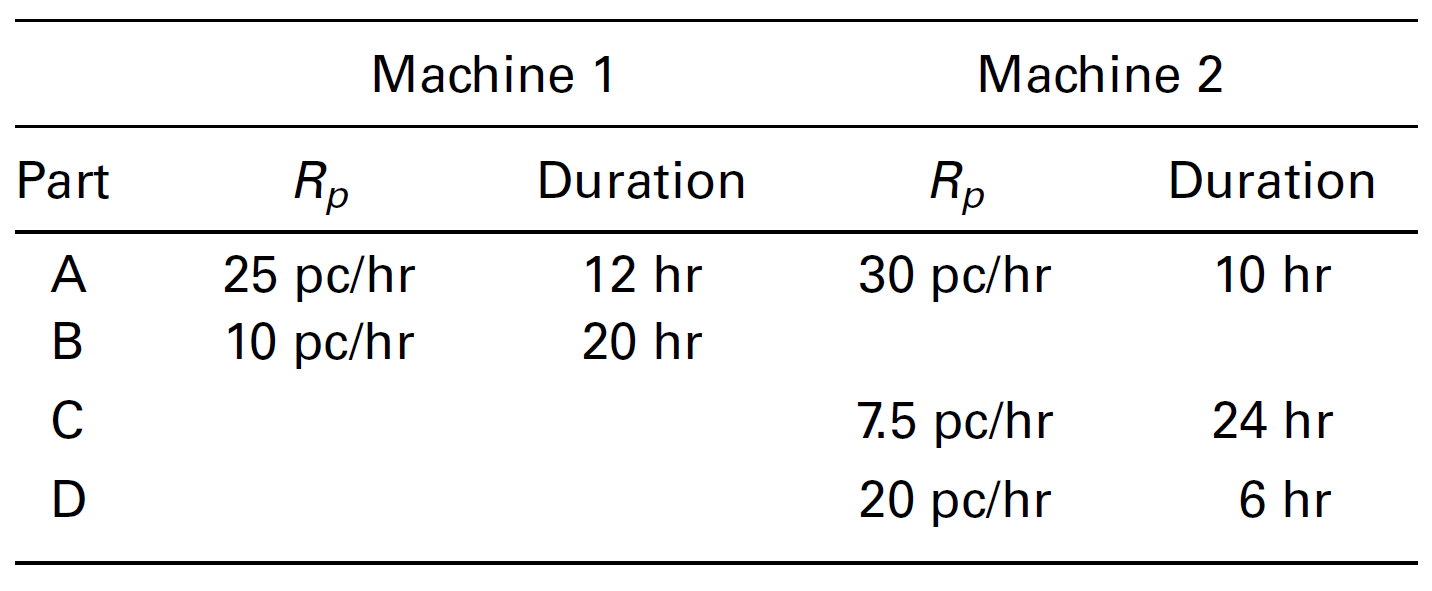
\includegraphics[scale=0.4]{img/example.png}
    \caption{Example of duration, $R_p$ for $n=2$ machines and 4 different styles $A-D$. The $WL$ is, in general the sum of the duration over all the machines $WL=12+20+10+24+6=72$, when used as plant capacity is the number of $H_{pw}$ multiplied by the number of machines, that is $WL=2\cdot{H_{pw}}=2\cdot{40}=80$}.
\end{figure}

\subsubsection{Manifacturing lead time ($MLT$)}
The \textit{Manifacturing Lead Time (MLT)} is the ttotale time required to process a part or a product through the plant, including any time due to delays, part being moved between operations and so on. Practically speaking it can be computed (by using average measures) as:
\begin{equation}
    MLT=n_o(T_{su}+Q{T_c}+T_{no}) 
\end{equation}
where $MLT$(min) is the average manifacturing lead time for \underline{all parts} in the plant, $T_{no}$ is the \textit{non-operation time}\footnote{
    One can wonder the reason why such non-operation times are present. There is the time for transporting one batch from one operation to another, the time lost for an issue in the equipment, the time spent in assembling queues of products and so on.
} 

\subsubsection{Work-In-Process ($WIP$)}
The $WIP$ (Work in process)\footnote{aka \textit{Work-in-progress}} (measured in pieces) is the total number of pieces which are present in a given firm. That is the product which are being processed or that are between processing operations. It can be defined as
\begin{equation}
    WIP=R_{pph} (MLT)
\end{equation} 
The pieces computed by analyzing $WIP$ cannot be transformed into revenue until all processing has been completed. The most desirable thing is that as soon is possible, all $WIP$ could be converted in revenue.

\subsection{\color{red} Manifacturing costs}
The decisions can be made about the automation of production systems can be made according to the \textbf{relative costs of alternatives}. In this chapter we are seeing how such costs, referred as \textit{manifacturing costs} are determined.\\
There are two main categories of manifacturing costs: 
\begin{enumerate}
    \itemsep-0.3em
    \item \textit{Fixed costs (FC)} which remains constant for any output level of the production plant; 
    \item \textit{Variable costs (VC)} are the ones varying according to the output of the plant.
\end{enumerate}
The total cost can be obtained as
\begin{equation}\label{eq:TC}
    TC=FC+VC(Q)
\end{equation}
where $Q$ is the output level. In order to evaluate some production methods, a useful thing is building a diagram of the production quantity vs the (total) costs. In fact, you can see in fact that \Cref{eq:TC} is a line in the variable $Q$.\\
\noindent
An alternative classification of manifacturing costs is the one individuating:
\begin{itemize}
    \itemsep-0.3em
    \item \textit{Direct labor} which are the salary for the workers; 
    \item \textit{Materials} comprise the cost for raw material/starting material; 
    \item \textit{Overhead} are all the other expenses associated with th firm which can be \textsf{Factory overhead} if those costs are related to the production, otherwise if they are related to the managing part, they are called \textsf{Corporate overhead}.
\end{itemize}

\begin{figure}
    \centering
    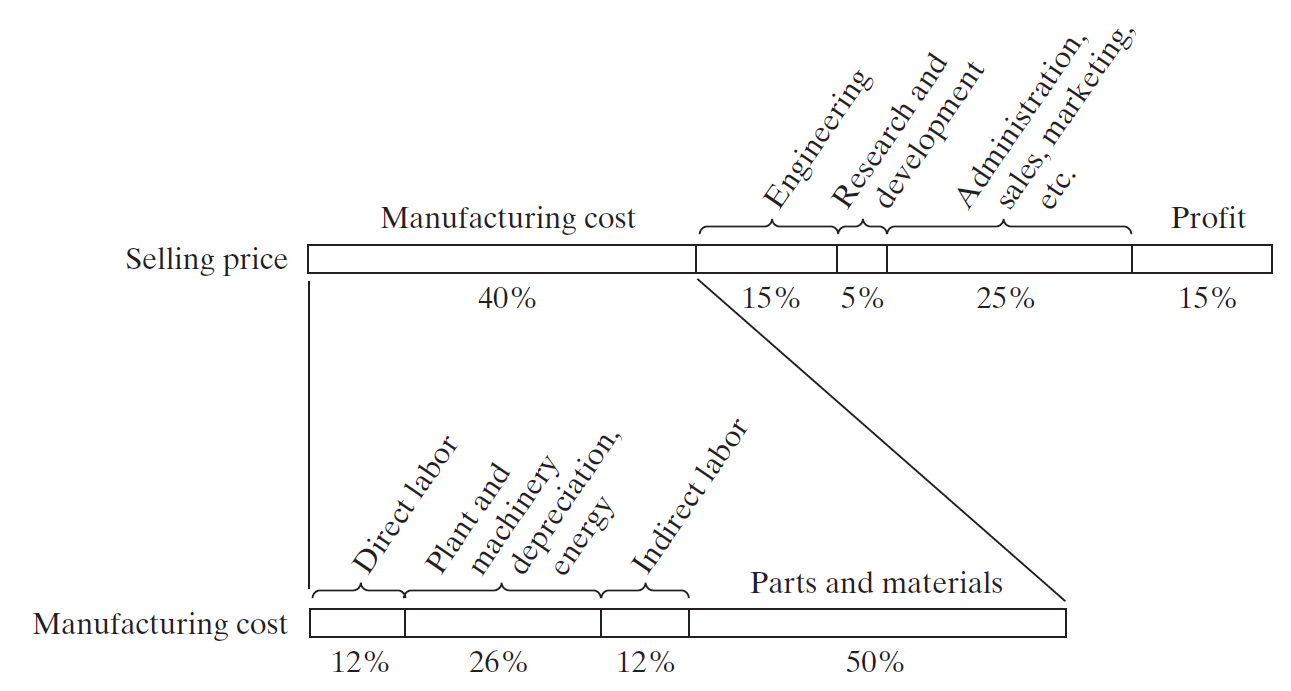
\includegraphics[scale=0.6]{img/costs_manufacturing.png}
    \caption{Breakdown of manifacturing costs}
    \label{fig:J_Black}
\end{figure}

The \Cref{fig:J_Black} shows a typical breakdown for selling price and manifacturing costs. Some overhead factors (tipically in percentage) can be computed in order to be able to estimate parameters like the selling price. Such factors are:
\begin{align}
    &FOHR=\frac{FOHC}{DLC}\qquad\text{Factory overhead rate}\\
    &COHR=\frac{COHC}{DLC}\qquad\text{Corporate overhead cost}
\end{align}
where $DLC$ is the direct labor cost.

\subsubsection{Cost of Equipment Usage}
An hourly cost of \textit{worker-machine} system is given by: 
\begin{equation}
    C_o=C_L(1+FOHR_L)+C_m(1+FOHR_m)
\end{equation}
where $C_o$ is the hourly rate (\$/hr), $C_L$ is the labor rate and $C_m$ is the machine rate while $FOHR_L$ and $FOHR_m$ are respectively the labor and machine factory overhead rate. 

\subsubsection{Cost of a Manifactured Part}
The cost for a manifactured part is defined as the sum of production cost, material cost and tooling cost. For a unit operation the cost is given by 
\begin{equation}
    C_{oi}T_{pi}+C_{ti}
\end{equation}
The cost for the final product/part is given by the sum of the material costs and unit costs:
\begin{equation}
    C_{pc}=C_m+\sum (C_{oi}T_{pi}+C_{ti})
\end{equation}
Where $C_{pc}$ is the cost per piece and $C_m$ is the cost per piece for starting/raw material.